\documentclass[]{article}

% Imported Packages
%------------------------------------------------------------------------------
\usepackage{amssymb}
\usepackage{amstext}
\usepackage{amsthm}
\usepackage{amsmath}
\usepackage{enumerate}
\usepackage{float}
\usepackage{fancyhdr}
\usepackage[margin=1in]{geometry}
\usepackage{graphicx}
%\usepackage{extarrows}
%\usepackage{setspace}
%------------------------------------------------------------------------------

% Header and Footer
%------------------------------------------------------------------------------
\pagestyle{plain}  
\renewcommand\headrulewidth{0.4pt}                                      
\renewcommand\footrulewidth{0.4pt}                                    
%------------------------------------------------------------------------------

% Title Details
%------------------------------------------------------------------------------
\title{Deliverable \#2 Template}
\author{SE 3A04: Software Design II -- Large System Design}
\date{}                               
%------------------------------------------------------------------------------

% Document
%------------------------------------------------------------------------------
\begin{document}

\maketitle	
\noindent{\bf Tutorial Number:} T0x\\
{\bf Group Number:} Gx \\
{\bf Group Members:} 
\begin{itemize}
	\item List all Group Member Names (as listed in Avenue)
	\item You do not need to use student \#s or macid (keep those private).
\end{itemize}

\section*{IMPORTANT NOTES}
\begin{itemize}
	%	\item You do \underline{NOT} need to provide a text explanation of each diagram; the diagram should speak for itself
	\item Please document any non-standard notations that you may have used
	\begin{itemize}
		\item \emph{Rule of Thumb}: if you feel there is any doubt surrounding the meaning of your notations, document them
	\end{itemize}
	\item Some diagrams may be difficult to fit into one page
	\begin{itemize}
		\item Ensure that the text is readable when printed, or when viewed at 100\% on a regular laptop-sized screen.
		\item If you need to break a diagram onto multiple pages, please adopt a system of doing so and thoroughly explain how it can be reconnected from one page to the next; if you are unsure about this, please ask about it
	\end{itemize}
	\item Please submit the latest version of Deliverable 1 with Deliverable 2
	\begin{itemize}
		\item Indicate any changes you made.
	\end{itemize}
	\item If you do \underline{NOT} have a Division of Labour sheet, your deliverable will \underline{NOT} be marked
\end{itemize}

\newpage
\section{Introduction}
\label{sec:introduction}
% Begin Section

This section should provide an brief overview of the entire document.

\subsection{Purpose}
\label{sub:purpose}
% Begin SubSection
State the purpose and intended audience for the document.
% End SubSection

\subsection{System Description}
\label{sub:system_description}
% Begin SubSection
Give a brief description of the system. This could be a paragraph or two to give some context to this document.

% End SubSection

\subsection{Overview}
\label{sub:overview}
% Begin SubSection
Describe what the rest of the document contains and explain how the document is organised (e.g. "In Section 2 we discuss...in Section 3...").

% End SubSection

% End Section

\section{Analysis Class Diagram}
\label{sec:analysis_class_diagram}
% Begin Section
This section should provide an analysis class diagram for your application.
% End Section


\section{Architectural Design}
\label{sec:architectural_design}
% Begin Section
This section should provide an overview of the overall architectural design of your application. Your overall architecture should show the division of the system into subsystems with high cohesion and low coupling.

\subsection{System Architecture}
\label{sub:system_architecture}
% Begin SubSection
\begin{itemize}
	\item Identify and explain the overall architecture of your system
	\item Be sure to clearly state the name of the architecture you used (this is the name of the architectural pattern, not the name of your system)
	\item Provide the reasoning and justification of the choice of architecture
	\item Provide a structural architecture diagram showing the relationship among the subsystems (if appropriate)
	\item List any design alternatives you considered, but eliminated (and explain why you eliminated them)
\end{itemize}

\begin{figure}[H]
	\centering
	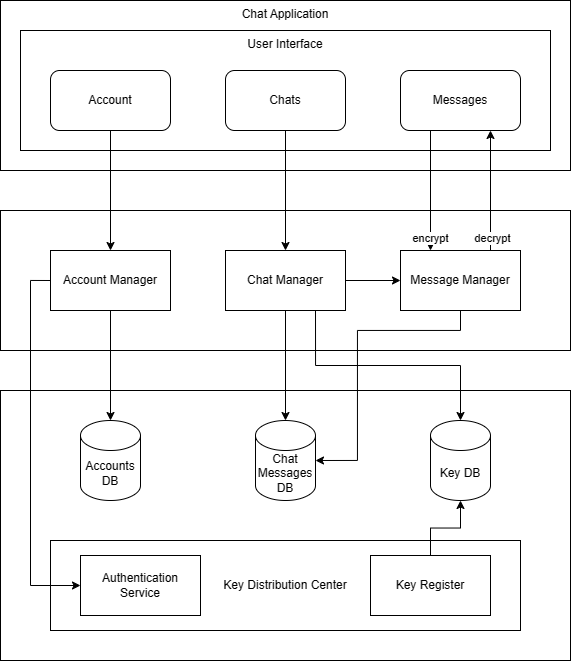
\includegraphics[width=1\textwidth]{architecture_diagram.drawio.png}
	\caption{System Architecture of the Project}
\end{figure}
% End SubSection

\subsection{Subsystems}
\label{sub:subsystems}
% Begin SubSection
 Provide a list of your subsystems, with a brief description of each. Be sure to document its purpose and relationship to other subsystems.

    The Account Manager subsystem is central to user management operations within the application. It handles tasks such as user authentication, creating new user accounts, and maintaining user data. It interfaces with the Accounts Database (DB), which stores user information securely. By managing user identities (UIDs) and related data, it serves as the backbone for user verification and is critical for maintaining user integrity and security within the application.

    The Chat Manager is responsible for managing the chat sessions. It enables users to view all their chats, add or remove participants, and also manages the encryption keys from the Key Distribution Center (KDC). By interfacing with the Chat Messages DB, it ensures that all chat data is accurately reflected in user sessions. This subsystem works closely with the Message Manager, providing the necessary keys for encryption and decryption of messages.

    Message Manager: Serving as the communication facilitator, the message manager is tasked with handling all aspects of message exchange. It stores, encrypts, and decrypts messages, ensuring they are securely sent to and from users within the chat. This subsystem interacts with Chat Manager subsystem to get the necessary encryption and decryption keys. This is crucial for maintaining the confidentiality of the messages. The Message Manager works in conjunction with the Chat Manager to ensure messages within a chat are properly secured and delivered to the intended recipients.

% End SubSection

% End Section
	
\section{Class Responsibility Collaboration (CRC) Cards}
\label{sec:class_responsibility_collaboration_crc_cards}
% Begin Section
This section should contain all of your CRC cards.

\begin{itemize}
	\item Provide a CRC Card for each identified class
	\item Please use the format outlined in tutorial, i.e., 
	\begin{table}[ht]
		\centering
		\begin{tabular}{|p{5cm}|p{5cm}|}
		\hline 
		 \multicolumn{2}{|l|}{\textbf{Class Name:}} \\
		\hline
		\textbf{Responsibility:} & \textbf{Collaborators:} \\
		\hline
		\vspace{1in} & \\
		\hline
		\end{tabular}
	\end{table}
	
\end{itemize}
% End Section

\appendix
\section{Division of Labour}
\label{sec:division_of_labour}
% Begin Section
Include a Division of Labour sheet which indicates the contributions of each team member. This sheet must be signed by all team members.
% End Section
\subsection{Awurama Nyarko}
\label{subsec:awurama_nyarko}
\begin{itemize}
	\item 1.1 Purpose
	\item 1.2 System Description
	\item 1.3 Overview
	\item 3.1 System Architecture: explained used of MVC and Repository
\end{itemize}
\includegraphics[width=0.5\textwidth]{awurama signaturec.jpg}

\subsection{Chelsea Maramot}
\label{subsec:chelsea_maramot}
\begin{itemize}
	\item Figure 1. Part of Analysis Class Diagram
	\item Class Responsibility Collaboration (CRC) cards
 		\begin{itemize}
   			\item File Management: File Error Handling
      			\item File Management: File Access
	 		\item File Management: File Search and Retrieval
    			\item Account Management: Account Management
       			\item Account Management: Account Database
	  		\item Account Management: User Information
     			\item Account Management: Log-in/Sign-in
			\item Account Management: Change Status
   			\item Account Management: View Account
      		\end{itemize}
\end{itemize}
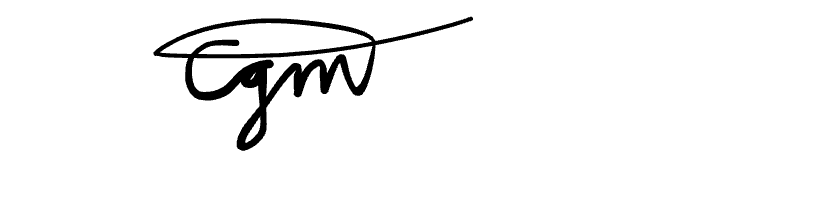
\includegraphics[width=0.5\textwidth]{chelsea.png}

\subsection{Harrison Chiu}
\label{subsec:harrison_chiu}
\begin{itemize}
	\item 3.1 System Architetcure: explained elimiation of other architecture designs
	\item Figure 2. System Architecture
 	\item 3.2 Subsystems
\end{itemize}

\includegraphics[width=0.5\textwidth]{harrison.png}

\subsection{Khushi Bhojane}
\label{subsec:khushi_bhojane}
\begin{itemize}
	\item Figure 1. Part of Analysis Class Diagram
	\item Class Responsibility Collaboration (CRC) cards
 		\begin{itemize}
   			\item Authentication Management: Encryption
      			\item Authentication Management: Token Generation
	 		\item Authentication Management: Authentication Management
    			\item Chat Management: Send Message
       			\item Chat Management: Send Files
	  		\item Chat Management: Edit/Delete Message
     			\item Chat Management: Disappearing/Vanishing Messages
			\item Chat Management: Load Previous Messages
   			\item Chat Management: 'Delivered' Status Message
      		\end{itemize}
\end{itemize}
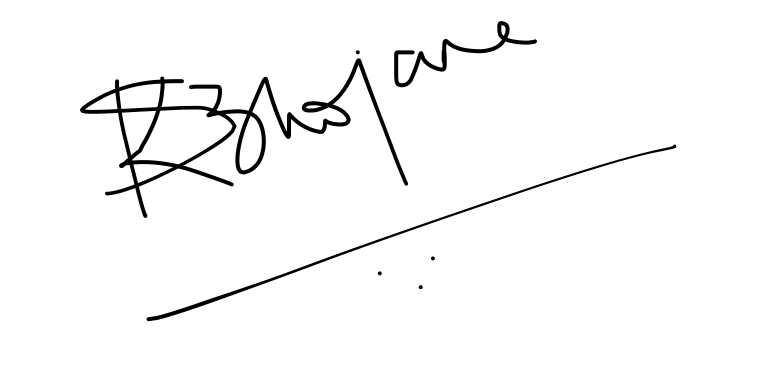
\includegraphics[width=0.5\textwidth]{khushi_signature.png}

\subsection{Sumanya Gulati}
\label{subsec:sumanya_gulati}
\begin{itemize}
	\item Figure 1. Part of Analysis Class Diagram
	\item Class Responsibility Collaboration (CRC) cards
 		\begin{itemize}
   			\item Chat Management: Chat History Database
      			\item Chat Management: Create Group
	 		\item Chat Management: Edit Group Members
    			\item Chat Management: Edit Group Details
       			\item Chat Management: Message Error
	  		\item Chat Management: Chat Management
     			\item File Management: File Management
			\item File Management: File Permissions
      		\end{itemize}
\end{itemize}

\includegraphics[width=0.5\textwidth]{signature.jpeg}

\end{document}
%------------------------------------------------------------------------------
